\documentclass[tikz, border=3.14mm]{standalone}
\usepackage{pgfplots}
\pgfplotsset{compat=1.18}
\usepgfplotslibrary{groupplots}

\begin{document}
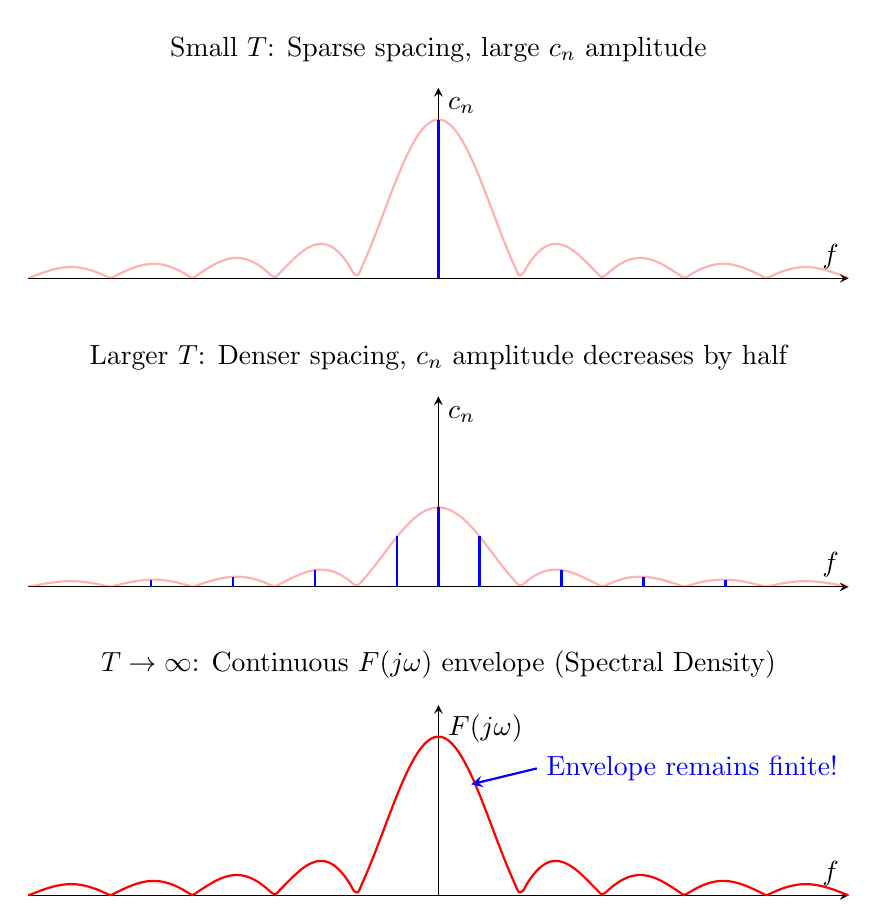
\begin{tikzpicture}
    \begin{groupplot}[
        group style={group size=1 by 3, vertical sep=1.5cm},
        axis lines = middle,
        xlabel = {$f$},
        ylabel = {$c_n$},
        xmin = -5, xmax = 5,
        ymin = 0, ymax = 1.2,
        xtick = \empty,
        ytick = \empty,
        width = 12cm,
        height = 4cm,
        domain = -5:5,
        samples = 200
    ]
        % Case 1: Small T (e.g. T=1), wide spacing, large cn
        \nextgroupplot[title={Small $T$: Sparse spacing, large $c_n$ amplitude}]
        \addplot[red, thick, smooth, opacity=0.3] {abs(sin(x*180/1)/(x*3.14))};
        \foreach \n in {-4,-2,0,2,4} {
            \edef\temp{\noexpand\addplot[blue, thick, ycomb] coordinates {(\n, {(\n == 0 ? 1 : abs(sin(\n*180/1)/(\n*3.14)))})};}
            \temp
        }

        % Case 2: Larger T (e.g. T=2), narrow spacing, smaller cn
        \nextgroupplot[title={Larger $T$: Denser spacing, $c_n$ amplitude decreases by half}]
        \addplot[red, thick, smooth, opacity=0.3] {0.5*abs(sin(x*180/1)/(x*3.14))};
        \foreach \n in {-8,-7,...,8} {
            \pgfmathsetmacro\val{0.5*\n}
            \edef\temp{\noexpand\addplot[blue, thick, ycomb] coordinates {(\val, {(\n == 0 ? 0.5 : 0.5*abs(sin(\val*180/1)/(\val*3.14)))})};}
            \temp
        }

        % Case 3: T -> inf, F(jw) envelope
        \nextgroupplot[title={$T \to \infty$: Continuous $F(j\omega)$ envelope (Spectral Density)}, ylabel={$F(j\omega)$}]
        \addplot[red, thick, smooth, domain=-5:5, samples=200] {abs(sin(x*180/1)/(x*3.14))};
        \node[anchor=west, blue] (note) at (axis cs:1.2, 0.8) {Envelope remains finite!};
        \draw[->, >=stealth, blue, thick] (note.west) -- (axis cs:0.4, 0.7);

    \end{groupplot}
\end{tikzpicture}
\end{document}
